Many dynamic engineering system design problems contain two groupings of the design variables: plant (or artifact) and control.
For instance, consider again the system-level design of a robotic manipulator presented in Chapter~\ref{ch:1}. The plant design may comprise the geometric properties of the links and the control design may be embodied by the joint torque time trajectories for a specific task~\cite{Allison2013d}.
Many authors have shown the benefit of a combined strategy rather than a sequential approach~\cite{Fathy2003a, Allison2014b, Deshmukh2016a, Yan2009a, Fathy2001a}.
With a sequential approach, the plant is optimized initially, followed by the controller~\cite{Fathy2001a, Allison2014a}. 
In this chapter, we focus on two solution strategies appropriate for combined plant and controller design or co-design: \textit{simultaneous} and \textit{nested}.

% new paragraph
The simultaneous solution strategy optimizes both the plant and control variables in same optimization formulation.
With the nested strategy, an outer optimization loop optimizes the plant design, and an inner optimization loop identifies the optimal control for each plant design tested by the outer loop~\cite{Fathy2001a, Allison2014a}.
These two strategies are selected for a few reasons beyond them being the most studied and used in the literature.
First, the simultaneous strategy is the most fundamental representation of an integrated design problem \cite{Martins2013a}. 
On the other hand, the nested strategy is a specific reorganization of the optimization problem based on the plant and control disciplines.
Multidisciplinary design optimization (MDO) is a field of research that investigates design methods for systems with multiple disciplines \cite{Martins2013a, Allison2014a}.
However, if we are limited to single-system problems and implementations that do not partition the system across trajectories, there are a limited number of appropriate MDO methods suitable for co-design.
One reason for this is that many MDO formulations were developed in a way that does not explicitly address the dynamic nature of general co-design problems \cite{Allison2014a}.
This has led to partitioning schemes without full consideration of the coupling in the system.
Allison and Nazari developed an augmented Lagrangian coordination method for co-design, but only accounted for unidirectional (plant) coupling \cite{Allison2010b}.
The nested approach naturally handles single-system problems, bidirectional coupling, and the various trajectories in the problem.
Another important motivating reason for reorganizing the original problem is to employ specialized optimization algorithms to solve specific subproblems \cite{Allison2010b, Kusiak1995a}.
A number of efficient solution methods for specific problem forms can be utilized with the nested strategy.
However, as it will be discussed throughout this article, both of these strategies have their drawbacks. 
Many of these issues are well known for simultaneous strategy, motivating the fields of MDO and distributed optimization \cite{Martins2013a}.
The nested strategy is not amenable to coarse-grained parallelism and can be computationally intensive \cite{Allison2010b}.
Additionally, it can have potential feasibility issues.

% new paragraph
Here we consider co-design problems that are well-posed as \glsfirst{DO} problems~\cite{Fathy2001a, Allison2014a, Herber2014a}.
Co-design theory has focused primarily on specific DO formulations; as a result, only limited types of co-design problems fit into the existing frameworks.
With a specific problem structure, a variety of algorithms have been developed to provide numerical solutions, and detailed analysis of the coupling and partitioning has been investigated~\cite{Fathy2001a, Frischknecht2011a, Reyer2001a, Hale1985a, Eastep1987a, Sunar1993a, Peters2011a, Peters2009a}.
Such works have made considerable progress towards addressing specific challenges found in certain co-design problems.
However, there has been less attention towards the general co-design problem (i.e.,~a co-design formulation with no restrictions) perhaps due to the lack of efficient solution techniques and continuing legacy design practices that treat certain problem elements as naturally separate~\cite{Allison2014a}. 

% new paragraph
Recently, numerical solution methods have been utilized to solve co-design problems that are not captured by previous problem definitions~\cite{Allison2014a, Herber2014a}.
Nontraditional problem formulation elements include system-level objective functions, general inequality path constraints, and general boundary conditions~\cite{Allison2013d, Allison2014b, Deshmukh2016a, Fathy2003a, Herber2013a, Maraniello2016a, Yan2009a, Chilan2017a}.
With these nontraditional problem elements, much of the previous work in co-design theory does not apply.
An essential element of engineering design optimization is an appropriate problem formulation.
A thorough analysis of the general co-design formulation is needed to better allow designers to leverage the advantages intrinsic to the co-design methodology.

% new paragraph
One of the numerical solution methods recently applied to co-design problems is known as \glsfirst{DT}, which approximates the infinite-dimensional DO problem with a finite \glsfirst{NLP} that can be solved with standard NLP solvers~\cite{Betts2010a, Biegler2010a, Rao2010a, Allison2014b}. 
DT has a number of favorable properties that supports the efficient generation of solutions to general co-design problems~\cite{Allison2014a, Allison2014b, Herber2014a}.

% new paragraph
In this chapter, we will explore the general co-design problem with a focus on the simultaneous and nested solution strategies.
Section~\ref{sec:ch3:formulation} provides the formulations for the simultaneous and nested co-design solution strategies and Sec.~\ref{sec:ch3:conditions} outlines the necessary conditions for optimality for both.
Section~\ref{sec:ch3:numerical} discusses some practical solution considerations relevant to the two strategies.
Section~\ref{sec:ch3:casestudies} presents a number of test problems and finally, Sec.~\ref{sec:ch3:conclusion} offers a summary.

\section{Problem Formulation \label{sec:ch3:formulation}}

Here we  present the two co-design strategies. First, we state a few assumptions. Initially, the time horizon $t_{\glsfirst{initial}} \leq \gls{time} \leq t_{\glsfirst{final}}$ is assumed to be fixed. Section~\ref{sec:ch3:time} discusses the inclusion of the horizon boundaries in the co-design problem formulations.
Next, only general inequality constraints will directly appear in the formulations for conciseness of the formulations. Equality constraints are captured by two inequality constraints (i.e.,~$\glsfirst{f}(\gls{x}) = 0$ is equivalent to $f(\bm{x}) \leq 0$ and $-f(\bm{x}) \leq 0$). % cite something?

\subsection{Simultaneous Formulation}

The general simultaneous co-design problem formulation contains all relevant objectives and constraints in a single optimization formulation. % AAO?
The DO problem formulation is:
\begingroup
\allowdisplaybreaks
\begin{subequations}
\label{eq:simprob}
\begin{align}
\min_{\bxp, \bxc} \quad & \Psi(\bxp, \bxc) = \int_{t_0}^{t_f} \lagrange \left( t, \bxi, \bxc, \bxp \right) dt \ + \cdots \label{eq:ch3:sim_lagrange} \\
& \qquad \mayer \left( \bxi(t_0), \bxi(t_f), \bxc, \bxp \right) \label{eq:ch3:sim_mayer} \\
\text{subject to:} \quad & \dot{\bxi \glsfirst{timederiv}} - \bfd \left( t, \bxi, \bxc, \bxp \right) = \bzero \label{eq:ch3:sim_codesign_dyn} \\
& \gls{path} \left( t, \bxi, \bxc, \bxp \right) \leq \bzero \label{eq:sim_codesign_path} \\
& \gls{boundary} \left( \bxi(t_0), \bxi(t_f), \bxc, \bxp \right) \leq \bzero \label{eq:ch3:sim_codesign_bound}
\end{align}
\end{subequations}%
\endgroup

\noindent where $\bm{x}_{\glsfoo[noindex]{plant}}$ are the plant variables, $\bm{x}_{\glsfoo[noindex]{control}}$ are the control variables, $t$ is the time continuum defined between $t_0$ and $t_f$, $\gls{states}$ are the states, $\gls{objective}$ is the objective function in Bolza form, \gls{lagrange} is the Lagrange (running cost) term, \gls{mayer} is the Mayer (terminal cost) term, Eqn.~(\ref{eq:ch3:sim_codesign_dyn}) enforces the dynamics modeled as a first-order ordinary differential equation, Eqn.~(\ref{eq:sim_codesign_path}) enforces any time-varying path constraints, and Eqn.~(\ref{eq:ch3:sim_codesign_bound}) enforces any time-dependent constraints. See Ref.~\cite{Herber2014a} for a general discussion of this co-design formulation and the problem elements.

\subsection{Nested Formulation}

The alternative solution strategy to the simultaneous formulation in Prob.~(\ref{eq:simprob}) is a nested one where an outer optimization loop optimizes the plant design, and an inner optimization loop identifies the optimal control for each plant design tested by the outer loop.
Figure~\ref{fig:ch3:strategies} illustrates the two strategies.
This is a two-level optimization problem (a subclass of bilevel optimization)~\cite{Colson2007a, Vicente1994a, Tanino1984a}. The outer-loop problem is defined as:
\begin{subequations}
\label{eq:ch3:outerloop}
\begin{align}
\min_{\bxp} \quad & \psi ( \bxp ) \qquad \qquad \qquad \label{eq:ch3:outerloop_obj}
\end{align}
\vspace*{-\baselineskip}
\begin{empheq}[right={\empheqrbrace = \bm{g}_{o} ( \bxp ) \leq \bm{0} }]{align}
\text{subject to:} \quad & \bm{\phi}_{o} \left( \bxp \right) \leq \bzero \label{eq:ch3:outerloop_phi} \\
& \bm{F}(\bxp) \leq \bm{0} \label{eq:ch3:outerloop_F}
\end{empheq}
\end{subequations}

\begin{figure}[t]
\centering
\begin{subfigure}[b]{0.3\columnwidth}
       \centering
       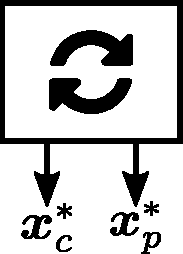
\includegraphics[width=0.46923076922in]{../ch3/figures/strategies_sim}
       \caption{Simultaneous strategy.\label{fig:ch3:strategies_sim}}
\end{subfigure}% 
\begin{subfigure}[b]{0.3\columnwidth}
       \centering
       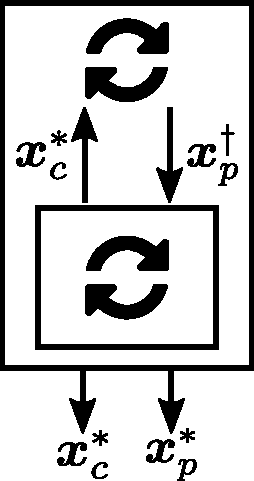
\includegraphics[width=0.65in]{../ch3/figures/strategies_nested}
       \caption{Nested strategy.\label{fig:ch3:strategies_nested}}
\end{subfigure}% 
\caption[Two co-design solution strategies]{Two co-design solution strategies where \faRefresh~indicates an optimization problem.\label{fig:ch3:strategies}}
\end{figure}

\noindent where $\bm{\phi}_{\glsfirst{outer}}$ are the constraints in $\bm{\phi}$ that only depend on the plant design, $\gls{inequality}_{o}$ is the collection of the outer-loop constraints, and $\{ \gls{objectiveouter} ( \bxp ), \gls{outerfeas}(\bxp) \}$ are two new problem formulation elements that will be outlined after the following inner-loop formulation:
\begin{subequations}
\label{eq:ch3:innerloop}
\begin{align}
\min_{\bxc} \quad & \Psi( \bxp^{\dagger}, \bxc) \qquad \qquad \qquad \qquad \qquad \quad
\end{align}
\vspace*{-\baselineskip}
\begin{empheq}[right={\empheqrbrace = \bm{g}_{i}\left( \cdot \right) \leq \bm{0} }]{align}
\text{subject to:} \quad &  \dot{\bxi} - \bfd \left( t, \bxi, \bxc, \bxp^{\dagger} \right) = \bzero \\
& \bm{C} \left( t, \bxi, \bxc, \bxp^{\dagger} \right) \leq \bzero \\
& \bm{\phi}_{i} \left( \bxi(t_0), \bxi(t_f), \bxc, \bxp^{\dagger} \right) \leq \bzero
\end{empheq}
\end{subequations}

\noindent where $\bxp^{\glsfirst{candidate}}$ is a candidate plant design, $\bm{\phi}_{\glsfirst{inner}}$ are the constraints of $\bm{\phi}$ not in $\bm{\phi}_{o}$, and $\bm{g}_{i}$ is the collection of the inner-loop constraints. With both formulations presented, some additional concepts relevant to two-level optimization problems need to be discussed.

% new paragraph
The simultaneous method's feasible set (or constraint region) is defined as:
\begin{align}
\gls{Omega} = \left\lbrace (\bxp, \bxc)\ :\ \bm{g}_{o}(\bxp, \bxc) \leq \bm{0}, \ \bm{g}_{i}(\bxp, \bxc) \leq \bm{0} \right\rbrace
\end{align}

\noindent For each candidate $\bxp^{\dagger}$, the inner-loop feasible set is defined by:
\begin{align}
\Omega(\bxp^{\dagger}) = \left\lbrace \bxc\ : \ \bm{g}_{i}(\bxp^{\dagger}, \bxc) \leq \bm{0} \right\rbrace
\end{align}

\noindent and then set of potential inner-loop optimal control designs is:
\begin{align}
\gls{Mcontrols}(\bxp^{\dagger}) = \left\lbrace \bxc\ :\ \bxc \in \arg\min \left\lbrace \Psi(\bxp^{\dagger}, \bxc)\ :\ \bxc \in \Omega(\bxp^{\dagger})  \right\rbrace \right\rbrace
\end{align}

\noindent For a given $\bxp$, $M(\bxp)$ may be empty for some values of its argument, i.e.,~no feasible control design exists for the given $\bxp$. If $\bxc \in M(\bxp)$, then the optimal objective function value from the inner loop is:
\begin{align}
\psi(\bxp) = \Psi(\bxp, \bxc)
\end{align}

\noindent which is used as the objective function of the outer loop, Eqn.~(\ref{eq:ch3:outerloop_obj}). Finally, the feasible set of the outer loop (known as the induced region) is:
\begin{align}
\gls{induced} = \left\lbrace (\bxp, \bxc)\ :\ (\bxp, \bxc) \in \Omega,\ \bxc \in M(\bxp) \right\rbrace
\end{align}

\noindent and we note that $\Omega$ and $I$ are not the same feasible region. This is the motivation behind the addition of Eqn.~(\ref{eq:ch3:outerloop_F}). $\bm{F}(\bxp)$ is an additional constraint that may be added to ensure for all $\bxp^{\dagger}$, $\Omega(\bxp^{\dagger})$ is nonempty, termed the outer-loop feasibility constraint. The two formulations are only equivalent if $\Omega$ remains unchanged. This constraint will be discussed more in the following discussion section.

\subsection{Formulation Discussion\label{sec:ch3:form_dis}}

Here we  discuss the specific problem formulation elements of both approaches, focusing on comparisons to the current co-design literature.

\subsubsection{Control Design Variables}

While plant variables will always be time-independent, control variables may be either time-independent or infinite-dimensional trajectories (with respect to time). We partition the control variables into two sets as:
\begin{align}
\bxc = \begin{bmatrix} \bp \\ \bu \end{bmatrix}
\end{align}

\noindent where \gls{parameters} are the control parameters and \gls{olc} are the \glsfoo[noindex]{OLC} variables.
The control parameters are static (time-independent) control variables (e.g.,~gains).
The OLC variables are infinite-dimensional trajectories through time (e.g.,~joint torque time profile for a robotic manipulator).
Both types of control design variables are found in the literature, although both types are not typically in the same design problem.
Even if there are no OLC variables, the general co-design problem is still an infinite-dimensional problem due to the dynamic and path constraints.
One very special case is when the optimal OLC can be defined with static gains such as with infinite-horizon \glsfirst{LQR}~\cite{Liberzon2012a, Belvin1990a, Rao1988a} discussed later in Sec.~\ref{sec:ch3:lqr}.
See Refs.~\cite{Belvin1990a, Eastep1987a, Fathy2003a, Rao1988a, Sunar1993a, Yan2009a} for examples with $\bp$ and Refs.~\cite{Allison2014b, Deshmukh2016a, Herber2013a, Maraniello2016a, Chilan2017a} for examples with $\bu$.

% paragraph about objective function
\subsubsection{Objective Function} 

Even though the objective function  is partitioned in Eqns.~(\ref{eq:ch3:sim_lagrange}) and (\ref{eq:ch3:sim_mayer}), converting between the Lagrange and Mayer terms is possible~\cite{Liberzon2012a, Herber2014a}. Both forms are present to allow for more natural formulations of the problem (and to be consistent with the literature).

A common form of the co-design objective function is:
\begin{align} \label{eq:ch3:sep_objs}
\min_{\bxp, \bxc} \quad \Psi = w_p \Psi_p ( \bxp ) + w_c \Psi_c\left( \bxp, \bxc \right)
\end{align}

\noindent where $\{\Psi_p, \Psi_c\}$ are the plant and control objective functions and $\{\gls{weights}_p, w_c\}$ are objective weights~\cite{Fathy2001a}. 
While many co-design problems are appropriately partitioned with control and plant specific objective function terms~\cite{Frischknecht2011a, Fathy2003a, Hale1985a, Peters2009a, Peters2011a, Rao1988a, Reyer2001a, Sunar1993a}, others necessitate the general objective form in Eqns.~(\ref{eq:ch3:sim_lagrange})--(\ref{eq:ch3:sim_mayer})~\cite{Allison2013d, Deshmukh2016a, Fathy2003a, Herber2013a, Chilan2017a}. 
These general objectives may only include one term or terms that are typically only classified as ``control'' objective terms.

\subsubsection{Path and Boundary Constraints}%
Equations~(\ref{eq:sim_codesign_path}) and (\ref{eq:ch3:sim_codesign_bound}) could be further generalized into a single general constraint form, but the distinction is important for both the optimality conditions and the numerical approaches used to find solutions.
The difference is primarily based on time dependence. Therefore, path and boundary constraints could be more appropriately named time-dependent and time-independent constraints.

% new paragraph
Boundary constraints are common to many existing co-design formulations~\cite{Fathy2001a, Allison2014a, Herber2014a}.
Traditional plant-only constraints such geometry or mass constraints are time-independent constraints~\cite{Peters2009a, Peters2011a, Allison2014b, Rao1988a}.
Many co-design formulations explicitly require initial condition constraints, but some co-design problems have unknown initial conditions or periodic constraints~\cite{Herber2013a}.
Another set of boundary constraints is the kinematic relationships in
robotics~\cite{Spong2005a}. These constraints might require an algebraic variable that depends on the states (e.g.,~the end position of the robotic manipulator depends on the state joint angles and geometric plant variables). 

% new paragraph
More recently, general path constraints have been included in co-design problems and are infinite-dimensional constraints~\cite{Herber2014a, Allison2014a, Allison2014b, Allison2013d}. 
Many traditional engineering constraints can be formulated naturally as path constraints.
States or outputs often need to be constrained between allowable bounds such as temperature, position, force, pressure, deflection, stress, power, etc. 
These examples are typically inequality path constraints but equality path constraints are also possible, such as an automobile following a prescribed drive cycle or ensuring the steady-state optimal tip-speed ratio is followed by a horizontal axis wind turbine~\cite{Deshmukh2016a}.
The inclusion of path constraints is critical to the usefulness of many co-design studies.
Fathy et al. included mixed control-plant constraints:
\begin{align}
\bm{C}\left(t, \bm{u}(t), \bm{x}_p \right) \leq \bm{0}
\end{align}
\noindent 
but mixed state-control-plant constraints as in Eqn.~(\ref{eq:sim_codesign_path}) are needed to represent many of the engineering constraints mentioned above~\cite{Fathy2001a}.

\subsubsection{Outer-Loop Feasibility Constraint}

For the two solution strategies to be equivalent, $M(\bxp)$ must be nonempty for every candidate $\bxp$~\cite{Fathy2001a}. Introducing an appropriate outer-loop feasibility constraint is one technique to ensure this property is satisfied.

% new paragraph
Consider again the design of a robotic manipulator. For certain geometric configurations, the kinematics restrictions of the manipulator may be such that it is unable to reach the prescribed target.
To avoid a candidate $\bxp$ that has no feasible control solution, we could add a reachability constraint to $\bm{F}(\bxp)$~\cite{Allison2013d, Spong2005a}.
However, even with this additional constraint, mixed state-control-plant constraints may be present that cannot be satisfied with the given plant design, such as stress or deflections~\cite{Allison2013d}.
This example helps illustrate that for general co-design problems, these constraints can be quite difficult (or impossible) to determine.

% new paragraph
An important type feasibility constraint is the classic controllability property applicable to linear systems theory~\cite{Fathy2001a}.
Unfortunately, controllability is not sufficient to guarantee the nonemptiness of $\Omega(\bxp^{\dagger})$ for general co-design problems.
For example, if control bounds are provided, then it is not guaranteed that we can move between arbitrary initial and final positions in finite time.

% new paragraph
It is also important to note that this outer-loop feasibility constraint may not strictly be required to find the system-optimal solution using the simultaneous strategy.
Another strategy is to add a feasibility constraint that restricts $\Omega$ such that the desired property holds.
This is not ideal since there will be no guarantee that the nested strategy will produce the system-level optimum, but may be a necessity for certain co-design problems.
The implications of this will be discussed in the following sections.

%---------------------------------------------------------------------
\section{Necessary Conditions for Optimality \label{sec:ch3:conditions}}

In this section, we describe the necessary conditions for optimality for the two general co-design strategies from the previous section. Sufficient conditions will not be discussed directly, but are the Hamiltonian minimization conditions~\cite{Liberzon2012a, Chachuat2007a, Bryson1975a} or second-order conditions on the Lagrangian for finite-dimensional problems~\cite{Papalambros2017a}.
If a problem is singular, there may be additional sufficient conditions needed~\cite{Chachuat2007a, Bryson1975a}.
We also assume that the simultaneous co-design problem is well-posed, i.e.,~there exists a solution. See Refs.~\cite{Liberzon2012a, Chachuat2007a, Papalambros2017a} for discussions on constraint qualification, regularity, differentiability, and other relevant properties for a well-posed problem.
We begin with the conditions for the OLC design only.

\subsection{Open-Loop Control Design}

The optimal OLC design problem formulation is:
\begingroup
\allowdisplaybreaks
\begin{subequations}
\label{eq:ch3:ocsd}
\begin{align}
\min_{\bu} \quad & \Psi = \int_{t_0}^{t_f} \lagrange \left( t, \bxi, \bu \right) dt + \mayer \left( \bxi(t_0), \bxi(t_f) \right) \\
\text{subject to:} \quad & \dot{\bxi} - \bfd \left( t, \bxi, \bu \right) = \bzero \label{eq:ch3:ocsd_2} \\
& \bm{C} \left( t, \bxi, \bu \right) \leq \bzero \label{eq:ch3:ocsd_3} \\
& \bm{\phi} \left( \bxi(t_0), \bxi(t_f) \right) \leq \bzero \label{eq:ch3:ocsd_4}
\end{align}
\end{subequations}
\endgroup

\noindent which is a subformulation of Prob.~(\ref{eq:simprob}).
Similar to the Lagrangian in finite-dimensional optimization~\cite{Papalambros2017a, Liberzon2012a}, the infinite-dimensional constraints can be adjoined to the Lagrange term with time-varying Lagrange multipliers, creating the Hamiltonian of the problem:
\begin{align}
\gls{hamiltonian} &= \lagrange + \blambda^{\glsfirst{transpose}} \bfd + \bmu\tran \bm{C}
\end{align}

\noindent where $\gls{costates}(t)$ are the costates (multipliers for the state dynamics) and $\gls{multiplierpath}(t)$ are the multipliers for $\bm{C}$.

% new paragraph
With this control-only formulation, we can directly apply \glsfirst{PMP} with path constraints~\cite{Pontryagin1962a, Liberzon2012a, Chachuat2007a} to arrive at the following necessary conditions for optimality (note, \glsname{optimal} is used to denote an optimal value):
\begin{subequations}
\label{eq:ch3:ocsd_cond}
\begin{gather}
\dot{\blambda}^* = - \left[ \pd{H}{\bxi} \right]^* \label{eq:ch3:ocsd_cond_1} \\
\bzero = \left[ \pd{H}{\bu} \right]^* \label{eq:ch3:ocsd_cond_2} \\
0 = \left[ \bmu\tran \bm{C}\right]^*, \quad 0 = \left[ \bnu\tran \bm{\phi} \right]^* \label{eq:ch3:ocsd_cond_3} \\
\bmu^* \geq \bzero, \quad \bnu^* \geq \bzero \label{eq:ch3:ocsd_cond_4} \\
\bzero = \left[ \blambda + \pd{\mayer}{\bxi} + \bnu\tran \pd{\bm{\phi}}{\bxi} \right]_{t_0}^* \label{eq:ch3:ocsd_cond_5}, \quad 
\bzero = \left[ \blambda - \pd{\mayer}{\bxi} - \bnu\tran \pd{\bm{\phi}}{\bxi} \right]_{t_f}^*
\end{gather}
\end{subequations}

\noindent where \gls{multiplierbound} are the Lagrange multipliers for $\bm{\phi}$,
Eqn.~(\ref{eq:ch3:ocsd_cond_1}) is the {costate dynamics},
Eqn.~(\ref{eq:ch3:ocsd_cond_2}) is the {control stationarity condition},
Eqns.~(\ref{eq:ch3:ocsd_cond_3}) are the {complementary slackness conditions},
Eqns.~(\ref{eq:ch3:ocsd_cond_4}) are the {dual feasibility conditions}, and
Eqns.~(\ref{eq:ch3:ocsd_cond_5}) are the {initial and final time transversality conditions}.
The conditions in Eqn.~(\ref{eq:ch3:ocsd_cond}) are in addition to the constraints in Eqns.~(\ref{eq:ch3:ocsd_2})--(\ref{eq:ch3:ocsd_4}). The necessary conditions for both strategies can now be derived.

\subsection{Co-design---Simultaneous Strategy}

Here we will derive the simultaneous co-design optimality conditions only using PMP.
Others have derived the optimality conditions for similar co-design formulations.
See Ref.~\cite{Dolezal1981a} for early work outside the co-design context.
Fathy et al. utilized a combination of the \glsfirst{KKT} conditions and PMP~\cite{Fathy2001a}.

% new paragraph
Consider the following augmented state vector:
\begin{align}
\label{eq:ch3:augmented_states}
\gls{augstate} = \begin{bmatrix} \bxi \\ \bxp \end{bmatrix}, \quad \dot{\bm{\Theta}} = \begin{bmatrix} \bfd \\ \bzero \end{bmatrix}
\end{align}

\noindent with the replacement of all plant variables with $\bxp(t_0)$ and, therefore, no dependence on $\bxp(t_f)$. Now consider if unconstrained, the choice of initial and final states are, in effect, additional decision variables that can be modified to satisfy the optimality conditions.

% new paragraph
The $\bm{\xi}$-dependent terms in Eqn.~(\ref{eq:ch3:ocsd_cond}) are Eqns.~(\ref{eq:ch3:ocsd_cond_1}) and (\ref{eq:ch3:ocsd_cond_5}). Applying these conditions to the ``state'' plant variables, we have the following additional conditions:
\begin{subequations}
\begin{align}
-\dot{\blambda}^*_p &= \left[ \pd{H}{\bxp} \right]^* = \left[ \pd{\lagrange}{\bxp}  + \blambda\tran \pd{\bfd}{\bxp} + \blambda_p\tran \cancelto{0}{\pd{\dot{\bm{x}}_p}{\bxp}} + \bmu\tran \pd{\bm{C}}{\bxp} \right]^*
  \\
\bzero &= \left[ \blambda_p + \pd{\mayer}{\bxp} + \bnu\tran \pd{\bm{\phi}}{\bxp} \right]_{t_0}^*  \\
\bzero &= \left[ \blambda_p - \cancelto{0}{\pd{\mayer}{\bxp}} - \bnu\tran \cancelto{0}{\pd{\bm{\phi}}{\bxp}} \quad \right]_{t_f}^* = \blambda_p^*(t_f)
\end{align}
\end{subequations}

\noindent Now using the first fundamental theorem of calculus, we can combine these equations into a single condition:
\begin{subequations}
\begin{gather}
\blambda^*_p(t_f) = \blambda^*_p(t_0) + \int_{t_0}^{t_f} \dot{\blambda}^*_p dt \\
\hspace*{-0.08in} \bzero = \left[ \pd{\mayer}{\bxp} + \bnu\tran \pd{\bm{\phi}}{\bxp} \right]_{t_0}^* + \int_{t_0}^{t_f} \left[ \pd{\lagrange}{\bxp}  + \blambda\tran \pd{\bfd}{\bxp} + \bmu\tran \pd{\bm{C}}{\bxp} \right]^* \hspace*{-0.07in} dt \label{eq:ch3:opt_cond_xp_codesign}
\end{gather}
\end{subequations}

\noindent This condition is analogous to the condition found in other derivations of the optimality conditions~\cite{Fathy2001a, Dolezal1981a}.
Note that the other conditions in Eqn.~(\ref{eq:ch3:ocsd_cond}) remain unchanged.
Therefore, the simultaneous co-design optimality conditions are a combination of Eqn.~(\ref{eq:ch3:ocsd_cond}) and Eqn.~(\ref{eq:ch3:opt_cond_xp_codesign}):
\begingroup
\allowdisplaybreaks
\begin{subequations}
\label{eq:ch3:opt_cond_sim}
\begin{gather}
\dot{\blambda}^* = - \left[ \pd{H}{\bxi} \right]^*, \quad 
\bzero = \left[ \pd{H}{\bu} \right]^* \\
0 = \left[ \bmu\tran \bm{C}\right]^*, \quad 0 = \left[ \bnu\tran \bm{\phi} \right]^*, \quad \bmu^* \geq \bzero, \quad \bnu^* \geq \bzero \\
\bzero = \left[ \blambda + \pd{\mayer}{\bxi} + \bnu\tran \pd{\bm{\phi}}{\bxi} \right]_{t_0}^*, \quad
\bzero = \left[ \blambda - \pd{\mayer}{\bxi} - \bnu\tran \pd{\bm{\phi}}{\bxi} \right]_{t_f}^* \\
\hspace*{-0.08in} \bzero = \left[ \pd{\mayer}{\bxp} + \bnu\tran \pd{\bm{\phi}}{\bxp} \right]_{t_0}^* + \int_{t_0}^{t_f} \left[ \pd{\lagrange}{\bxp}  + \blambda\tran \pd{\bfd}{\bxp} + \bmu\tran \pd{\bm{C}}{\bxp} \right]^* \hspace*{-0.07in}  dt
\end{gather}
\end{subequations}
\endgroup

\subsection{Co-design---Nested Strategy}

We now derive the necessary conditions for the nested strategy where the outer-loop problem is defined in Prob.~(\ref{eq:ch3:outerloop}) and the inner loop in Prob.~(\ref{eq:ch3:innerloop}).
The inner-loop optimality conditions are defined in Eqn.~(\ref{eq:ch3:ocsd_cond}) with only OLC variables.
If the inner loop contains $\bp$, then the necessary conditions are analogous to the simultaneous conditions in Eqn.~(\ref{eq:ch3:opt_cond_sim}) with $\bp$ replacing $\bxp$.

% new paragraph
The outer-loop problem is finite-dimensional optimization since neither the dynamics nor path constraints are present. Therefore, we can directly utilize the KKT conditions~\cite{Papalambros2017a}. The Lagrangian for the outer-loop problem is:
\begin{align}
L = \psi + \gls{multiplierouter}\tran \bm{\phi}_o + \gls{multiplierfeas}\tran \bm{F}
\end{align}

\noindent We first express the stationarity condition:
\begin{subequations}
\label{eq:ch3:nested_stationarity}
\begin{align}
\bzero = \der{L}{\bxp} &= \der{\psi}{\bxp} + \bm{\chi}\tran \der{\bm{\phi}_o}{\bxp} + \bm{\eta}\tran \der{\bm{F}}{\bxp} \\
&= \int_{t_0}^{t_f} \der{\lagrange}{\bxp} dt + \der{\mayer}{\bxp} + \bm{\chi}\tran \der{\bm{\phi}_o}{\bxp} + \bm{\eta}\tran \der{\bm{F}}{\bxp}
\end{align}
\end{subequations}

\noindent Now the total derivative terms can be explicated~\cite{Weisstein2016a}:
\begin{subequations}
\begin{align}
\der{\lagrange}{\bxp} &= \pd{\lagrange}{\bxp} + \pd{\lagrange}{\bxi^*}  \der{\bxi^*}{\bxp} + \pd{\lagrange}{\bu^*} \der{\bu^*}{\bxp} + \pd{\lagrange}{\bp^*} \der{\bp^*}{\bxp} \\
\der{\mayer}{\bxp} &= \pd{\mayer}{\bxp} + \left[ \pd{\mayer}{\bxi^*}  \der{\bxi^*}{\bxp} \right]_{t_0} + \left[ \pd{\mayer}{\bxi^*}  \der{\bxi^*}{\bxp} \right]_{t_f} + \pd{\mayer}{\bp^*}  \der{\bp^*}{\bxp} \label{eq:ch3:total_der_mayer}
\end{align}
\end{subequations}

\noindent Here we see a number of coupled terms.

% new paragraph
The complete set of necessary conditions for the outer loop are then:
\begin{subequations}
\label{eq:ch3:nested_cond}
\begin{gather}
\bzero = \der{\Psi}{\bxp} + \bm{\chi}\tran \der{\phi_o}{\bxp} + \eta\tran \der{F}{\bxp} \\
\bm{\chi} \geq \bzero, \quad \bm{\eta} \geq \bzero, \quad 
\bm{\chi}\tran \bm{\phi}_o = \bzero, \quad \bm{\eta}\tran \bm{F} = \bzero
\end{gather}
\end{subequations}

\noindent which are a set of KKT conditions. The conditions in Eqn.~(\ref{eq:ch3:nested_cond}) are in addition to the constraints Eqns.~(\ref{eq:ch3:outerloop_phi}) and (\ref{eq:ch3:outerloop_F}).

\subsection{Free Time \label{sec:ch3:time}}

The initial and final time values can be optimization variables as well~\cite{Liberzon2012a, Chachuat2007a, Fathy2001a, Herber2014a}.  
Optimal control problems frequently contain these terms and therefore, appropriate optimality conditions are provided.
Subsequently, these additional optimization variables are typically included in the inner-loop problem of the nested co-design strategy~\cite{Fathy2001a}. 
However, some of the numerical methods used jointly with certain co-design strategies lose certain properties when the time horizon is not fixed.
In these situations, perhaps, it is more beneficial to place these additional variables in the outer loop to maintain such properties.

The simultaneous co-design strategy will need one additional equation if $t_f$ is free:
\begin{align}
0 = \left[\pd{\mayer}{t_f} + \bnu\tran \pd{\bm{\phi}}{t_f} \right]^* + \left[ \lagrange + \blambda\tran \bfd + \bmu\tran \bm{C} \right]^*_{t_f}
\end{align}

\noindent This is an additional transversality condition with the others in Eqn.~(\ref{eq:ch3:ocsd_cond_5})~\cite{Liberzon2012a, Chachuat2007a}.

For a nested approach with $t_f$ free in the outer loop, the additional stationary condition $d L / d t_f = 0$ would include: 
\begin{subequations}
\begin{align}
\der{\lagrange}{t_f} &= \pd{\lagrange}{t_f} + \pd{\lagrange}{\bxi^*}  \der{\bxi^*}{t_f} + \pd{\lagrange}{\bu^*} \der{\bu^*}{t_f} + \pd{\lagrange}{\bp^*} \der{\bp^*}{t_f} \\
\der{\mayer}{t_f} &= \pd{\mayer}{t_f} + \left[ \pd{\mayer}{\bxi^*}  \der{\bxi^*}{t_f} \right]_{t_0} + \left[ \pd{\mayer}{\bxi^*}  \der{\bxi^*}{t_f} \right]_{t_f} + \pd{\mayer}{\bp^*}  \der{\bp^*}{t_f}
\end{align}
\end{subequations}

This completes the necessary conditions for optimality for the various problem formulations and solution strategies.
Now some of the computational and practical aspects will be discussed.

%---------------------------------------------------------------------
\section{Practical Solution Considerations \label{sec:ch3:numerical}}

Obtaining solutions only using the optimality conditions in the previous section can be challenging. Practical formulation limitations, robustness, and computational efficiency also need to be considered when seeking solutions to co-design problems.

\subsection{Obtaining Approximate Solutions \label{sec:ch3:approx}}

In the previous section,  the finding an analytic solution that satisfies the optimality conditions is called an indirect method~\cite{Betts2010a, Biegler2010a}. Although this approach can lead to important insights into the structure of the solution, it can be quite challenging (or impossible) to solve these equations analytically.
If complicated black box functions or table interpolation is used, analytic forms for their derivatives do not even exist.
Therefore, numerical methods are often employed that provide approximate solutions to the original problem.

% new paragraph
Numeric indirect methods derive explicitly the optimality conditions and then use discretization to form a \glsfirst{BVP}~\cite{Biegler2010a}.
If inequality path constraints are present, multiple BVPs will need to be linked for each arc that a path constraint is active since a new set of differential algebraic equations will need to be solved. 
The number of constrained subarcs and the sequence of constrained/unconstrained arcs, however, are unknown a priori, so it is quite difficult or even impossible to construct the correct BVP.

% new paragraph
Another issue with numeric indirect methods is standard solution procedures are not robust.
An initial guess for the costates must be given, but these are not physical quantities, so there typically is no good way of providing a reasonable estimate~\cite{Betts2010a}.
Furthermore, even with a reasonable guess, the numerical solution of the costate dynamics in Eqn.~(\ref{eq:ch3:ocsd_cond_1}) can be very ill-conditioned~\cite{Bryson1975a}.

% new paragraph
An alternative is direct methods~\cite{Biegler2010a, Betts2010a}. 
Instead of stating the optimality conditions, the control and/or state are parametrized using function approximation and the objective function is approximated using numerical quadrature.
This creates a discrete, finite-dimensional problem that then is optimized using large-scale NLP solvers~\cite{Biegler2010a}.

% new paragraph
The first class of direct methods is the sequential methods, which only parametrize the control.
Given initial conditions and a set of control parameters, the \glsfirst{DAE} model is solved through conventional DAE solvers (forward simulation) such as a Runge-Kutta method. 
Due to the use of conventional DAE solvers, this approach has the advantage of easily finding feasible solutions to the state equations, but needs to perform a full simulation for each perturbation in the optimization algorithm.
Repeated numerical integration of the DAE model, however, does not guarantee convergence with open-loop unstable systems~\cite{Biegler2010a} and the resulting solution can be very sensitive to the choice of control.
This strategy is the easiest to construct out of all the direct methods since reliable and efficient codes for DAE and NLP solvers are naturally linked~\cite{Biegler2010a}.

% new paragraph
Sequential approaches typically produce low-accuracy solutions and are computationally inefficient.
Many of these issues are due to the inability to handle path and boundary constraints efficiently.
Since the states are calculated through a forward simulation, we must approximate numerically how local control perturbations will affect the global state trajectory. This leads to simultaneous approaches that forgo the nested analysis of sequential methods for a large set of constraints\footnote{The sequential and simultaneous methods in this section are entirely different than the sequential design method mentioned at the beginning of this chapter and the simultaneous co-design method~\cite{Allison2014a, Allison2014b, Biegler2010a}. The methods in this section find approximate solutions to DO problems. The design methods are alternative solution methods for problems with plant and control design variables. For example, one could pose a simultaneous co-design problem and solve it with a sequential method for dynamic optimization.}.

\subsubsection{Direct Transcription \label{sec:ch3:dt}}

The simultaneous approach, also as known as direct transcription (DT), parametrizes both the state and control trajectories. 
Direct transcription is the focus in Chapter~\ref{ch:5} so it is only discussed briefly in the context of its usefulness in solving co-design problems.
Most DT methods are represented by the following NLP formulation:
\begingroup
\allowdisplaybreaks
\begin{subequations}
\begin{align}
\hspace*{-0.05in} \min_{\bm{U},\bm{\Xi}, \bxp} \ \  & \sum_{k=0}^{N_t} w_k \lagrange \left( t_k, \bxi(t_k), \bu(t_k), \bxp \right) + \mayer \left( \bxi(t_0), \bxi(t_f), \bxp \right) \label{eq:ch3:dt_1} \\
\text{subject to:} \quad & \bm{\zeta}\left( \bm{t}, \bm{\Xi}, \bm{U}, \bxp \right) = \bzero \label{eq:ch3:dt_2} \\
& \bm{C} \left( \bm{t}, \bm{\Xi}, \bm{U}, \bxp \right) \leq \bzero \label{eq:ch3:dt_3} \\
& \bm{\phi} \left( \bxi(t_0), \bxi(t_f), \bxp \right) \leq \bzero \qquad \qquad \qquad \qquad \label{eq:ch3:dt_4}
\end{align}
\end{subequations}
\endgroup

\noindent where $N_{\glsfirst{timesub}}+1$ is the number of discrete time points and $\left\lbrace \gls{distime}, \gls{disstate}, \gls{discontrol} \right\rbrace$ are the discretized forms of the time, states, and controls. The Lagrange term is approximated with numerical quadrature with weights $w_k$. The dynamic constraint is now enforced through a large number of equality constraints \gls{defect}, termed defect constraints~\cite{Rao2010a, Betts2010a, Biegler2010a}. Also, path constraints are now no more complicated than the dynamic constraints, a key advantage over other solution methods~\cite{Biegler2010a, Herber2015a}.

% new paragraph
This new large NLP formulation has a specific structure and sparsity pattern that can be exploited in NLP solvers to reduce total computational effort~\cite{Biegler2010a}. Simultaneous approaches have been shown to have good convergence properties and handle unstable DAEs~\cite{Biegler2007a, Garg2011a}. Finally, these approaches have specific advantages for singular control problems and high-index path constraints~\cite{Biegler2007a}. This collection of desirable properties makes DT a strong candidate for finding solutions to general co-design problems.

% new paragraph
General overviews of DT theory is available in Refs.~\cite{Biegler2010a, Betts2010a, Biegler2007a, Rao2010a, Allison2014b, Herber2014a}. Please see Refs.~\cite{Allison2014b, Allison2014a, Herber2014a} for further discussion on using DT to find solutions to co-design problems. In these co-design studies, DT was demonstrated to be a suitable method for finding solutions to more general co-design problems.

\subsection{Specific Forms}

In this chapter, we have presented the most general form of the co-design problem: both a nonlinear plant outer-loop and nonlinear control inner-loop.
However, specific forms of the control subproblem have been utilized heavily in a variety of co-design studies.
The primary motivation for these forms is the efficient generation of solutions for the inner-loop subproblem. These two forms are linear-quadratic dynamic optimization and LQR.

\subsubsection{Linear-Quadratic Dynamic Optimization}

Consider the following specific form of the control subproblem in Prob.~(\ref{eq:ch3:ocsd}):
\begingroup
\allowdisplaybreaks
\begin{subequations}
\label{eq:ch3:qp}
\begin{align}
\min_{\bu} \quad & \int_{t_0}^{t_f} \left( \begin{bmatrix} \bxi \\ \bu \end{bmatrix}\tran \begin{bmatrix} {\bm{Q}} & {\bm{N}} \\ {\bm{N}} & {\bm{R}} \end{bmatrix} \begin{bmatrix} \bxi \\ \bu \end{bmatrix} + \begin{bmatrix} {\bm{q}} \\ {\bm{r}} \end{bmatrix}\tran \begin{bmatrix} \bxi \\ \bu \end{bmatrix} \right) dt + \cdots \label{eq:ch3:dt_qp_1} \\
& \quad  \left[ \bxi\tran {\bm{M}} \bxi + {\bm{m}}\tran \bxi \right]_{t_0} + \left[ \bxi\tran {\bm{S}} \bxi + {\bm{s}}\tran \bxi \right]_{t_f} \label{eq:ch3:dt_qp_2}  \\
\text{subject to:} \quad & \dot{\bxi} - \left( \gls{dynA} \bxi + \gls{dynB} \bu + \gls{dynd} \right) = \bzero \\
& {\bm{C}}_1 \bxi + {\bm{C}}_2 \bu - {\bm{C}}_3 \leq \bzero \\
& {\bm{\phi}}_1 \bxi(t_0) + {\bm{\phi}}_2 \bxi(t_f) - {\bm{\phi}}_3 \leq \bzero
\end{align}
\end{subequations}%
\endgroup

\noindent where $t_f$ is finite and any of the matrices (with the exception of $\{\bm{\phi}, \bm{M}, \bm{m}, \bm{S}, \bm{s}\}$) can be time-varying.
This particular linear-quadratic DO problem can be approximated as a finite-dimensional \glsfirst{QP} using a DT method\footnote{A more general form of Prob.~(\ref{eq:ch3:qp}) is present in Chapter~\ref{ch:5} along with the methods for generating the QP using DT.}. Both single-step and pseudospectral DT methods can generate sparse QPs for this problem form~\cite{Herber2014a, Biegler2010a}.
Under certain conditions, the QP is convex and efficient to solve for even large systems and the global optimal solution for $\bm{u}$ is guaranteed.

% new paragraph
This form has been utilized in a number of nested co-design studies~\cite{Herber2014a, Chilan2017a}.
The simultaneous strategy cannot be applied with this form since most (if not all) co-design dynamic constraints have a nonlinear dependence on the optimization variables~\cite{Fathy2001a}. For example consider the following bilinear dynamic constraint: $\dot{\xi} = - k \xi$, where $k$ is a plant optimization variable. This dynamic constraint would need to be approximated with quadratic constraints.

\subsubsection{Linear-Quadratic Regulator \label{sec:ch3:lqr}}

Consider the following special form of the control-only subproblem: Prob.~(\ref{eq:ch3:qp}) containing only time-invariant matrices $\{ {\bm{Q}} \succeq 0, {\bm{R}} \succ 0, {\bm{A}}, {\bm{B}} \}$, no path constraints, simple initial value constraints ($\bm{\xi}(t_0) = \bm{\xi}_0$), and is infinite-horizon ($t_f \to \infty$). The optimal OLC can then be readily computed with the solution of the \glsfirst{ARE}:
\begin{align}
\label{eq:ch3:are}
\bm{P} {\bm{A}} + {\bm{A}}\tran \bm{P} - \bm{P} {\bm{B}} {\bm{R}}^{-1} {\bm{B}}\tran \bm{P} + {\bm{Q}} = 0
\end{align}

\noindent where \gls{dynP} is the unique, positive definite solution and $\bm{u}$ is:
\begin{align}
\bm{u}^* = - {\bm{R}}^{-1} {\bm{B}}\tran \bm{P}^* \bm{\xi}^*
\end{align}

\noindent This problem form is known as the infinite-horizon, continuous-time LQR~\cite{Liberzon2012a, Belvin1990a, Rao1988a}, and is quite heavily utilized in co-design studies~\cite{Rao1988a, Belvin1990a, Eastep1987a, Fathy2003a, Sunar1993a}.
Solutions of this form can be computed efficiently and have a number of favorable properties such as a closed-form solution that can be used to create an equivalent simultaneous formulation~\cite{Fathy2001a}. 
There are additional forms (e.g.,~finite-time and time-varying versions) of this type of problem~\cite{Bryson1975a, Liberzon2012a} but the computation cost quickly becomes comparable with highly structured QPs using DT solution methods. % reference?
However, this problem structure is simply unsatisfactory in addressing the requirements for some co-design problems (see Sec.~\ref{sec:ch3:form_dis}). 

\subsection{Comparing the Strategies}

A natural question is what solution technique should be used? This section will discuss some of the research around this question.

\subsubsection{Computation Time}

Here we parameterize the solution time for each method with:
\begin{subequations}
\begin{align}
\qquad \tau_s &= T_{0} + N T_{i} &\text{(simultaneous)} \\
 \qquad  \qquad \tau_n &= T_{0} + \bar{N} \left( \bar{T}_{i} + t_{0} + n t_{i} \right)  &\text{(nested)}
\end{align}
\end{subequations}

\noindent where $N$ is the number of optimization algorithm iterations needed for convergence, $T$ is a time variable, $n$ is the number of inner-loop iterations, $t$ is inner-loop time, $\bar{\Box}$ is an outer-loop quantity, $\Box_0$ is the initial time used to construct the optimization problem, and $\Box_i$ is the average iteration time.

% new paragraph
Obviously, if $\bar{N} > N$ and $\bar{T}_i > T_i$, then the simultaneous approach is superior, but this is unlikely as the nested strategy reduces the number of variables and constraints in the outer-loop problem.
This does highlight the computational goal of the nested approach.
Ideally we seek a nested strategy that significantly reduces both the number of iterations and time required during each iteration in the outer-loop, while keeping the time required to solve the nested subproblem small.

% new paragraph
Methods for reducing total computational expense for the general co-design problem with respect to either solution strategy are limited (other than favoring DT over other methods).
One suggestion from Ref.~\cite{Kelly2015a} is to treat plant variables in the simultaneous approach with DT exactly as in Eqn.~(\ref{eq:ch3:augmented_states}), where there is a plant variable at each time point and they are all constrained to be equal (which keeps Jacobian of the constraints and objective function sparse).
The development of guidelines and methods to help address the computational cost for different classes of co-design problems is left as future work.

\subsubsection{Literature-Based Recommendations}

Reyer et al. stated that the size and complexity of the simultaneous problem formulation could make this strategy impractical~\cite{Reyer2001a}.  
A number of authors have agreed with this statement, i.e.,~the nested strategy was better suited for their particular problem~\cite{Onoda1987a, Belvin1990a, Deshmukh2016a,Chilan2017a}.
In the case of Refs.~\cite{Onoda1987a, Belvin1990a}, the studies utilize the LQR for an extremely efficient inner loop, i.e.,~$t_0 + n t_i$ was quite small.
In Ref.~\cite{Deshmukh2016a}, there was an extreme computational expense associated with changes in the plant variables ($T_i$ was large), hence minimizing the number of function calls was paramount.
In Ref.~\cite{Chilan2017a}, there was both a high computational expense for modifying the plant design and the inner-loop could be solved with a QP.

% new paragraph
There are a limited set of studies that claim the opposite. 
In Ref.~\cite{Allison2014b}, the authors state that the simultaneous strategy is better, but the inner-loop was not solved with a QP even though it was in the Prob.~(\ref{eq:ch3:qp}) class, so it is hard to fairly compare the strategies.
However, it is still hard to make general recommendations since it is not very common for co-design study to compare the tradeoffs between the simultaneous and nested strategies for their particular design problem. In most design studies, only one strategy is needed if it is producing the desired results.

% new paragraph
There are some circumstances where the simultaneous strategy might be preferred.
For some problems, it might be the only viable method. For example, it may be impossible to separate the domains if black-boxes are used.
Also, consider the discussion of an empty $\Omega$ for a particular candidate plant design.
In this situation, the nested strategy could struggle or fail to find the optimal solution.
Another point is that the nested strategy does not follow the steepest descent direction in the simultaneous formulation (since the control variables are optimal for the control subproblem).
A simultaneous approach may better utilize the coupling between the plant and control design variables for faster convergence.

% new paragraph
It remains future work to determine if there are conditions such that a well-behaved simultaneous co-design formulation becomes more challenging to solve with the nested strategy.

\section{Test Problems \label{sec:ch3:casestudies}}

In this section, three co-design test problems (abbreviated \glsname{TP}) are defined which highlight some of the general co-design theory concepts\footnote{The \textsc{Matlab} codes for these test problems is available in Ref.~\cite{github-co-design-examples-repository}.}.
Please see also Refs.~\cite{Allison2013d, Allison2014b, Deshmukh2016a, Fathy2003a, Herber2013a, Maraniello2016a, Yan2009a, Chilan2017a} for examples of complex co-design problems that utilize nontraditional problem elements in the general co-design problem class.

\subsection{Test Problem 1: Scalar Plant, Scalar Control }

The first TP belongs to many early co-design formulations~\cite{Sunar1993a, Fathy2001a} including infinite time horizon, optimization of control gains, no path constraints, and separate control and plant objectives as in Eqn.~(\ref{eq:ch3:sep_objs}). The co-design problem is stated as:
\begin{subequations}
\begin{align}
\min_{b, K} \quad & \frac{w_c}{\xi_0^2} \int_{0}^{\infty} \left( q \xi^2 + r u^2  \right) dt + w_p b \\
\text{subject to:} \quad & \dot{\xi} = -b\xi + u \\
& \textcolor{light-gray}{\phi_1 := }\  \xi(0) - \xi_0 = 0 \\
& \textcolor{light-gray}{\phi_2 := }\  -b \leq 0, \ \textcolor{light-gray}{\phi_3 := }\ -K \leq 0
\end{align}
\end{subequations}

\noindent where $u = - K \xi$, $b \in \bxp$, and $K \in \bxc$. The results are shown in Fig.~\ref{fig:ch3:T2_1} for one particular set of values of the problem parameters. 

\begin{figure}[t!]
\centering
\begin{subfigure}[b]{0.4\columnwidth}
       \centering
        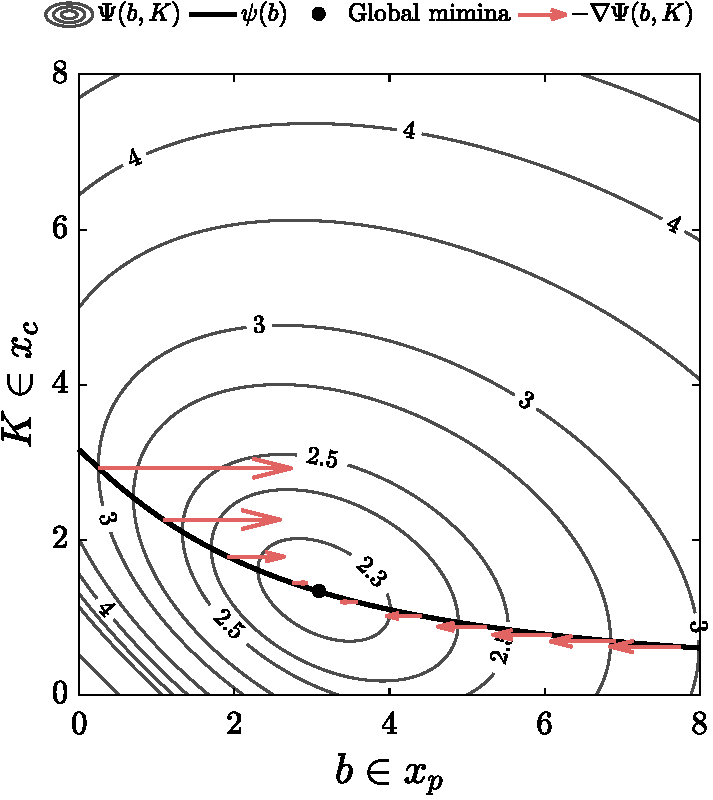
\includegraphics[width=\textwidth]{../ch3/figures/T2_1_PSI}
        \caption{$\Psi(b,K)$.\label{fig:ch3:T2_1_PSI}}
\end{subfigure}% 
\begin{subfigure}[b]{0.266666666667\columnwidth}
       \centering
        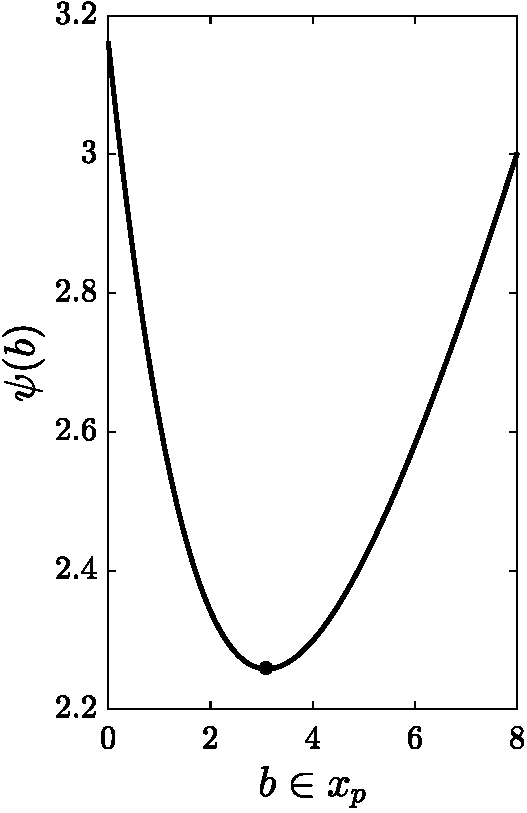
\includegraphics[width=\textwidth]{../ch3/figures/T2_1_nested}%
        \vspace{0.03in}
        \caption{$\psi(b)$.\label{fig:ch3:T2_1_nested}}
\end{subfigure}%
\caption[Scalar plant, scalar control problem (TP1) results]{Scalar plant, scalar control problem (TP1) results with $q=10$, $r=1$, $w_c = 1$, and $w_p = 0.3$.\label{fig:ch3:T2_1}}
\end{figure}


% new paragraph
For this problem, the ARE defined in Eqn.~(\ref{eq:ch3:are}) is a single quadratic equation: $0 = q - 2 b P - P^2/r$. The solution to this equation defines the gains of a full-state feedback optimal control law and therefore can be used to obtain the potential inner-loop optimal control designs, $M(\bxp)$, in a nested formulation. This is visualized in Fig.~\ref{fig:ch3:T2_1_PSI} as the solid black curve. We note that this is a subspace of $\Omega$, or simultaneous feasible set.
Comparing Fig.~\ref{fig:ch3:T2_1_PSI} and Fig.~\ref{fig:ch3:T2_1_nested}, we can visualize directly the difference between $\Psi(\bxp,\bxc)$ and $\psi(\bxp)$. We also note that the gradient of the nested solution trajectory in Fig.~\ref{fig:ch3:T2_1_PSI} is always orthogonal to the $K$-axis since it is the optimal gain value for a given $b$. 

% new paragraph
The coupling between the plant and control design variables is also present, noting the ``tilt'' of the level sets. Therefore, a sequential method would not be guaranteed to arrive at the global optima (but an iterative sequential strategy would in TP1)~\cite{Fathy2001a}.
In TP1, from all starting conditions, both the simultaneous and nested solution strategies arrive at the global optimum.
Although this is an extremely simple co-design problem, it does help visualize a number of important concepts.

%----------------------------
% this is the figures for TP2
\begin{figure*}
\centering

\begin{subfigure}[b]{1\textwidth}
       \centering
        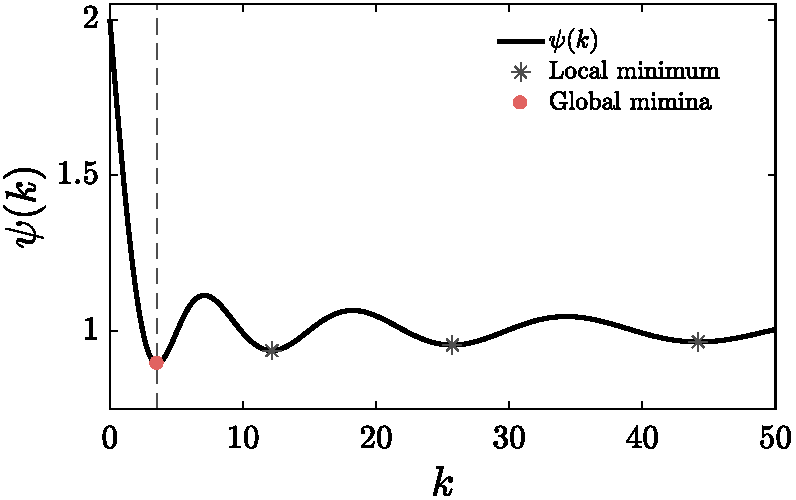
\includegraphics[width=0.333\textwidth]{../ch3/figures/T1_1_PSI}%
        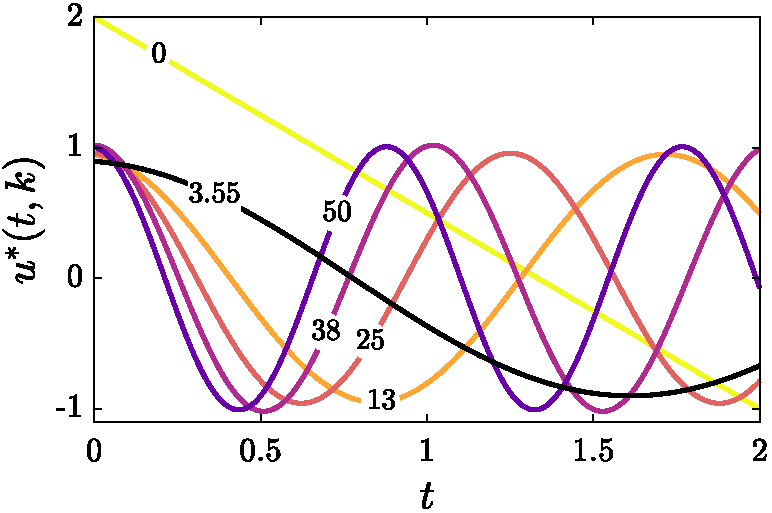
\includegraphics[width=0.333\textwidth]{../ch3/figures/T1_1_U}%
        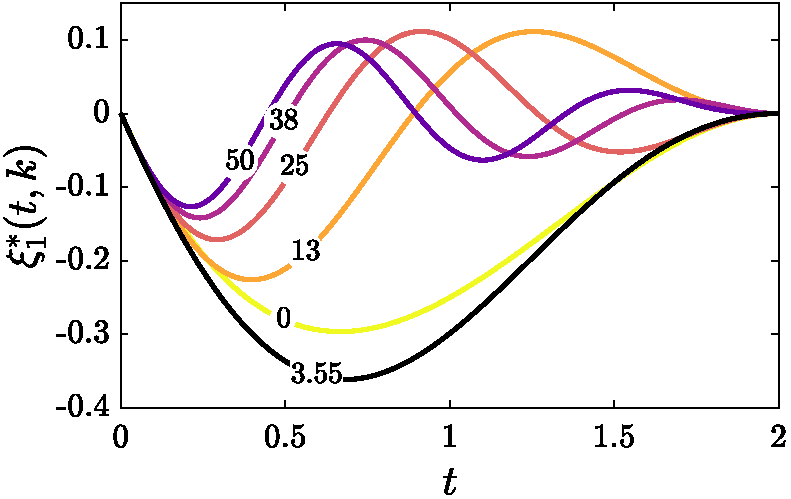
\includegraphics[width=0.333\textwidth]{../ch3/figures/T1_1_X}%
        \caption{TP2 results demonstrating a large number of
local solutions with $t_f = 2$, $x_0 = 0$, and $v_0 = -1$ (different values of $k$ marked).\label{fig:ch3:T1_1}}
\end{subfigure}%

\begin{subfigure}[b]{1\textwidth}
  \centering
  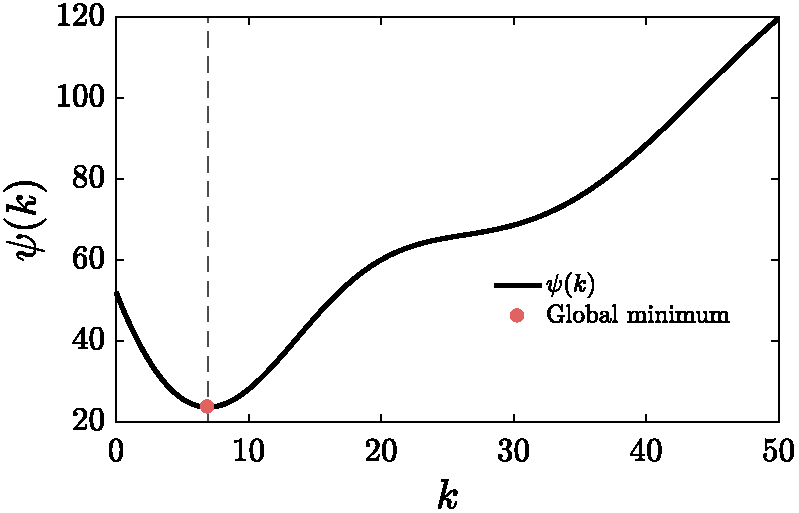
\includegraphics[width=0.333\textwidth]{../ch3/figures/T1_2_PSI}%
  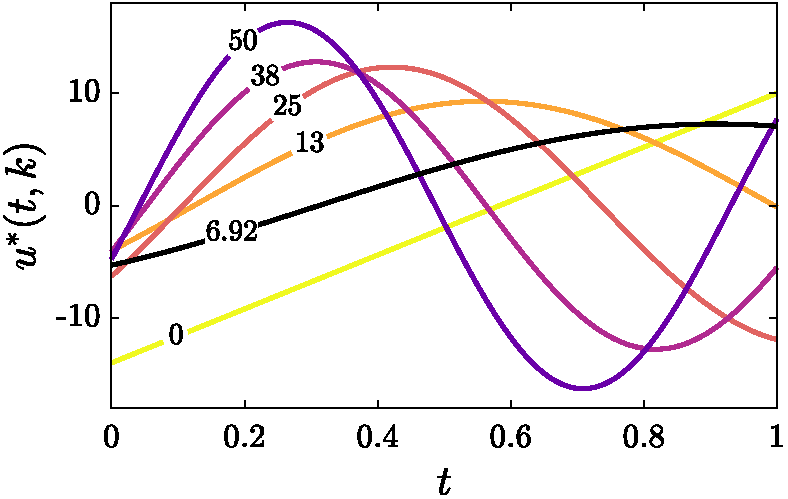
\includegraphics[width=0.333\textwidth]{../ch3/figures/T1_2_U}%
  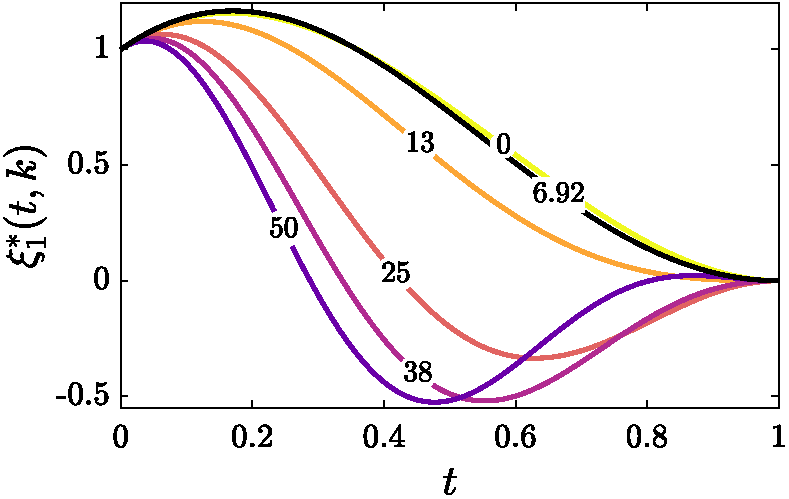
\includegraphics[width=0.333\textwidth]{../ch3/figures/T1_2_X}%
  \caption{TP2 results demonstrating single global minimum with $t_f = 1$, $x_0 = 1$, and $v_0 = 2$ (different values of $k$ marked).\label{fig:ch3:T1_2}}
\end{subfigure}%

\begin{subfigure}[b]{1\textwidth}
  \centering
  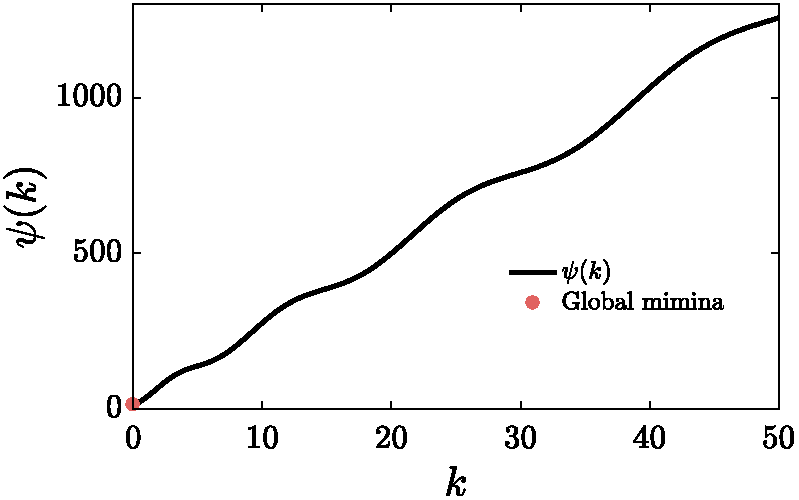
\includegraphics[width=0.333\textwidth]{../ch3/figures/T1_3_PSI}%
  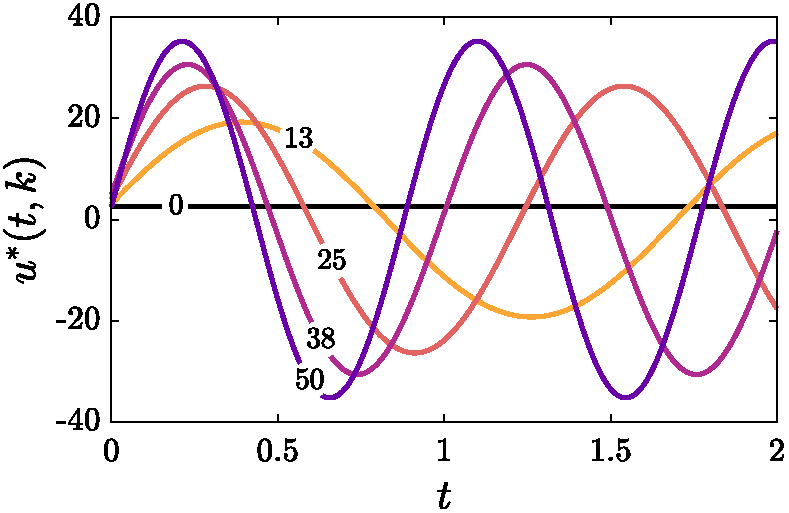
\includegraphics[width=0.333\textwidth]{../ch3/figures/T1_3_U}%
  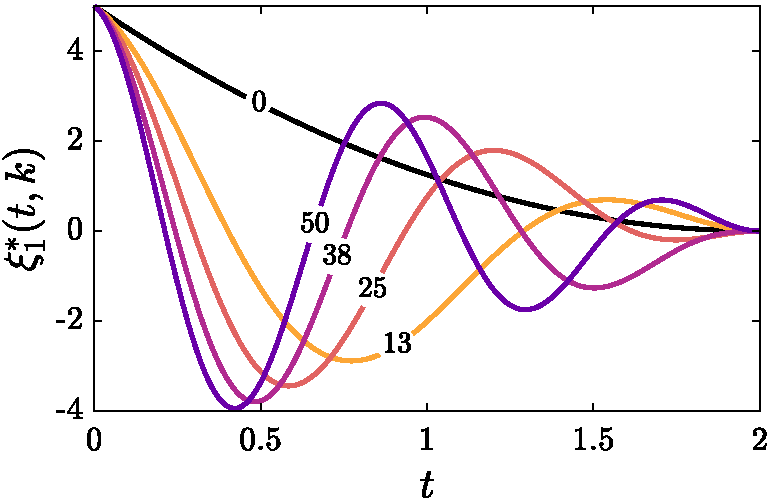
\includegraphics[width=0.333\textwidth]{../ch3/figures/T1_3_X}%
  \caption{TP2 results demonstrating degenerate plant solution with $t_f = 2$, $x_0 = 5$, and $v_0 = -5$ (different values of $k$ marked).\label{fig:ch3:T1_3}}
\end{subfigure}%

\caption[Co-design transfer problem (TP2) results]{Co-design transfer problem (TP2) results for various values of the problem parameters.\label{fig:ch3:T1}}
\end{figure*}% 
% moved here for positioning purposes
%----------------------------

%-----------------------------------------------------------------------------
\subsection{Test Problem 2: Co-Design Transfer \label{sec:ch3:transfer}}

Consider the following simple co-design problem that seeks to move a second-order system from an arbitrary initial state to rest while minimizing control effort:
\begin{subequations}
\begin{align}
\min_{k,u(t)} \quad & \int_{0}^{t_f} u^2 dt \\
\text{subject to:} \quad & \dot{\bxi} = \begin{bmatrix} 0 & 1 \\ -k & 0 \end{bmatrix}\bxi + \begin{bmatrix} 0 \\ 1 \end{bmatrix} u \\
& \textcolor{light-gray}{\phi_1 := }\ \xi_1(0) - x_0 = 0, \ \textcolor{light-gray}{\phi_2 := }\  \xi_2(0) - v_0 = 0 \\
& \textcolor{light-gray}{\phi_3 := }\ \xi_1(t_f) = 0, \ \textcolor{light-gray}{\phi_2 := }\  \xi_2(t_f) = 0
\end{align}
\end{subequations}

\noindent where $k\in \bm{x}_p$ and $u(t) \in \bm{x}_c$.
The solution for $u^*(t,k)$ (i.e.,~the nested strategy) can be obtained by scaling the problem~\cite{Herber2017c} into an equivalent DO problem in Ref.~\cite[pp.~166--167]{Bryson1975a} (details of this procedure are in Sec.~\ref{sec:ch4:transfer}):
\begingroup
\allowdisplaybreaks
\begin{subequations}
\label{eq:ch3:ex2_usol}
\begin{align}
u^*(t,k) &= - \frac{2k}{k t_f^2 - \sin^2(\sqrt{k} t_f)} \left( c_1(t,k) x_0 + c_2(t,k) \frac{v_0}{\sqrt{k}} \right) \\
c_1(t,k)  &= \sin\left( \sqrt{k}(t_f - t) \right)\sin\left(\sqrt{k}t_f\right) - \sqrt{k} t_f \sin \left(\sqrt{k}t \right) \\
c_2(t,k)  &= - \cos\left(\sqrt{k}(t_f-t)\right) \sin\left(\sqrt{k}t_f\right) + \sqrt{k} t_f \cos\left(\sqrt{k}t\right)
\end{align}%
\end{subequations}%
\endgroup

\noindent If $k=0$, then the solution above is not valid and $u^*$ is linear with respect to $t$. The original objective function can now be computed analytically by integrating the square of Eqn.~(\ref{eq:ch3:ex2_usol}). With this closed-form expression for the objective function, an optimality condition for $k$ can be derived using Eqn.~(\ref{eq:ch3:nested_stationarity}).

% new paragraph
The results for this TP are shown in Fig.~\ref{fig:ch3:T1} for various values of the problem parameters.
In Fig.~\ref{fig:ch3:T1_1}, there are a large number of local solutions of $\psi(k)$ and a clear global minimum at $k^*=3.554$.
In Fig.~\ref{fig:ch3:T1_2}, for the different values of the problem parameters, there is a single global minimum at $k^*= 6.924$.
Finally in Fig.~\ref{fig:ch3:T1_3}, there is a global minimum with $k^*=0$, i.e.,~the plant solution is degenerate.

% new paragraph
From these results, it is clear that caution should be used when claiming a global optimal co-design solution is found. Global search algorithms could improve the confidence of finding the true optimal solution such as a multistart approach or genetic algorithms~\cite{Papalambros2017a}. 
The control solution in Eqn.~(\ref{eq:ch3:ex2_usol}) demonstrates the complicated nature of the analytical solutions for even the simplest of co-design problems.
This problem may be a particularly useful TP as it is a well-posed co-design problem with a single system-level objective, general boundary conditions, and a closed-form OLC solution.

%-----------------------------------------------------------------------------
\subsection{Test Problem 3: Simple SASA}

The final TP is a co-design problem that was used directly in a detailed co-design study.
The co-design study focused on developing a novel \glsfoo[noindex]{SASA} system for spacecraft pointing control and jitter reduction~\cite{Chilan2017a} (please see Sec.~\ref{sec:ch4:sasa} for a detailed discussion of the connections to the detailed study in Chapter~\ref{ch:7}). Both the geometric properties of the solar array and OLC voltages along the array were the design variables.
To help provide some insight into the results of the original design study, a much simpler, but still representative, co-design problem was proposed:
\begin{subequations}
\label{eq:ch3:sasa_prob2}
\begin{align}
\min_{k,u(t)} \quad & - \xi_1(t_f) \\
\text{subject to:} \quad & \dot{\bm{\xi}} = \begin{bmatrix} 0 & 1 \\ -k/J & 0 \end{bmatrix} \bm{\xi} + \begin{bmatrix} 0 \\ 1/J \end{bmatrix} u \\
& \textcolor{light-gray}{\phi_1 := }\ \xi_1(0) = 0, \quad \textcolor{light-gray}{\phi_2 := }\  \xi_2(0) = 0 \\
& \textcolor{light-gray}{\phi_3 := }\  \xi_2(t_f) = 0 \\ 
& \textcolor{light-gray}{C_1 := }\  u - u_{\max} \leq 0, \quad \textcolor{light-gray}{C_2 := }\ -u - u_{\max} \leq 0
\end{align}
\end{subequations}

\begin{figure*}[t]
\centering
\begin{subfigure}[b]{0.333\textwidth}
       \centering
        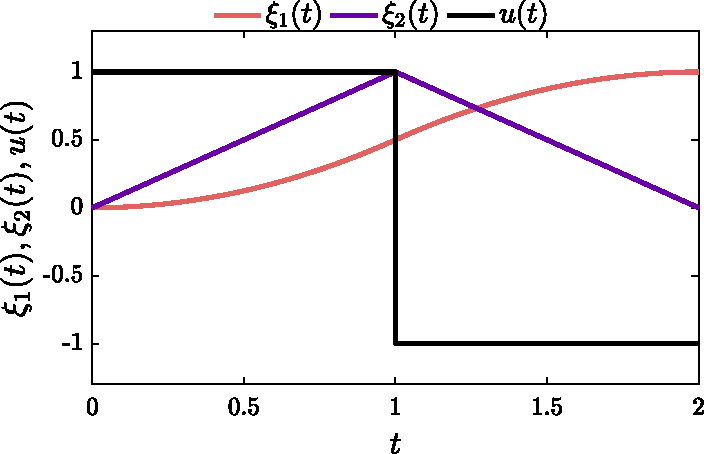
\includegraphics[width=\textwidth]{../ch3/figures/sasa_1.pdf}
        \caption{$k=0$.\label{fig:ch3:sasa_1}}
\end{subfigure}% 
\begin{subfigure}[b]{0.333\textwidth}
       \centering
        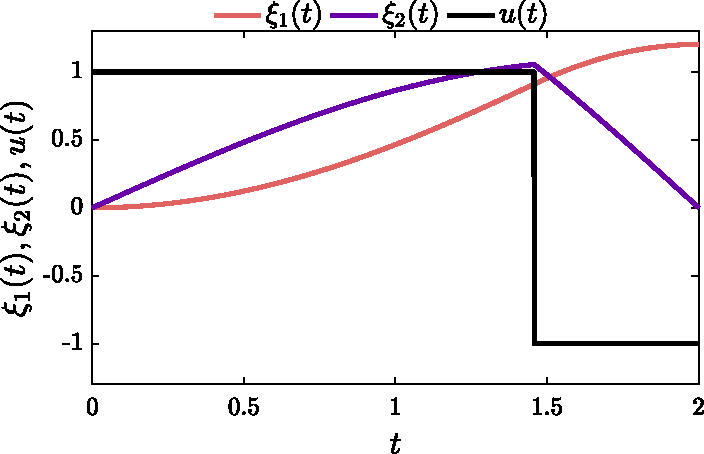
\includegraphics[width=\textwidth]{../ch3/figures/sasa_2.pdf}
        \caption{$k^*=0.8547$.\label{fig:ch3:sasa_2}}
\end{subfigure}%
\begin{subfigure}[b]{0.333\textwidth}
       \centering
        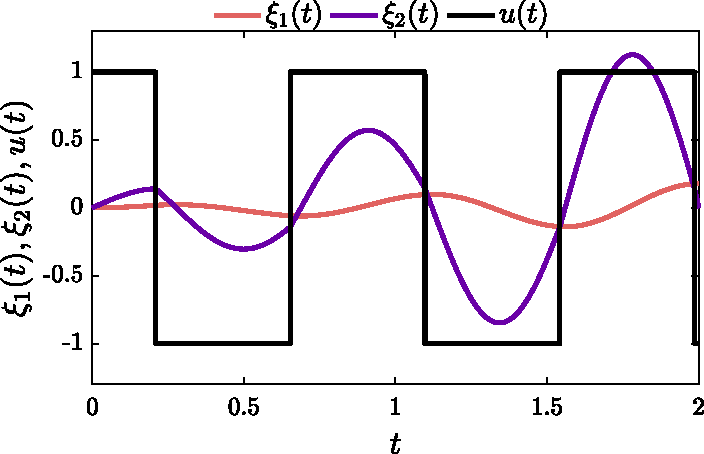
\includegraphics[width=\textwidth]{../ch3/figures/sasa_3.pdf}
        \caption{$k=50$.\label{fig:ch3:sasa_3}}
\end{subfigure}%
\caption[Simple SASA test problem (TP3) results]{Simple SASA test problem (TP3) results with $J=1$, $t_f=2$, and $u_{\max}=1$.\label{fig:ch3:sasa}}
\end{figure*}

\noindent where $k \in \bm{x}_p$  and $u(t) \in \bm{x}_c$. The results for this problem are shown in Fig.~\ref{fig:ch3:sasa} for various values of $k$ including $k^* = 0.8547$.

The OLC exhibits bang-bang behavior~\cite{Bryson1975a, Liberzon2012a}, i.e.,~$u$ is at either the minimum or maximum value. 
Using the control stationarity condition in Eqn.~(\ref{eq:ch3:ocsd_cond_2}), we can show directly that the Hamiltonian is minimized if $u$ exhibits bang-bang behavior, but determining the locations of the switching is quite challenging.
In a nested strategy, the number and location of the switches vary for different values of $k$ (see Fig.~\ref{fig:ch3:sasa_3} containing five switches while the optimal co-design solution only contains one switch in Fig.~\ref{fig:ch3:sasa_2}). This is a direct example of the discussion in Sec.~\ref{sec:ch3:approx} motivating the using of DT in co-design (see Sec.~\ref{sec:ch3:dt}).
The nested co-design solutions were found using DT formulated as a QP with both the composite quadrature and defect constraints based on the trapezoidal rule~\cite{Biegler2010a, Betts2010a, Herber2014a}.

% new paragraph
TP3 is an attractive TP as the closed-form solution for the simultaneous strategy can be computed to a high degree of accuracy, and it exhibits challenging behavior associated with inequality path constraints.

%---------------------------------------------------------------------
\section{Summary \label{sec:ch3:conclusion}}

In this chapter, general combined plant and controller design (or co-design) problems were examined.
A large portion of existing co-design theory has focused on specific DO formulations, leaving many open questions for co-design studies that do not fit the previous definitions. 

% new paragraph
There are two basic co-design solution strategies: simultaneous and nested.
The problem formulations for both strategies wer{}e presented and a discussion of the formulation elements was provided.
The nested strategy was presented as two-level optimization problem including a characterization of the differences in the feasibility region between the two strategies.
This motivated the outer-loop feasibility constraint as one approach for ensuring that for every candidate plant design, the control subproblem is well-posed.

% new paragraph
The natural next step was the presentation of the optimality conditions for both methods.
For the simultaneous strategy, the optimality conditions were derived using only Pontryagin's minimum principle and an augmented state vector.
Due to a number of challenges associated with the optimality conditions, practical solution considerations were discussed with a focus the motivating reasons for using DT in co-design (e.g.,~the activity of inequality path constraints).
Finally, three test problems were presented.
These problems were fairly simple but highlighted a number of key concepts including coupling, the difference between the feasible regions for each strategy, general boundary conditions, inequality path constraints, system-level objectives, and complexity of the closed-form solutions.

% new paragraph
This chapter seeks to provide a foundation for additional advances in general co-design theory. 
The outer-loop feasibility constraint warrants further investigation. 
Better comparisons between the two strategies are needed, especially for co-design problems without a specific form of the inner loop.
Developing methods for reducing total computational expense is also an important area such as the suggestion in Ref.~\cite{Kelly2015a} for treating plant variables like dummy states (or control) or alternative general strategies such decentralized optimization \cite{Allison2010b, Liu2017a}.
Finally, development of test problems that are more realistic could help answer some of the open questions.